%-------------------------------------------------------------------------------
% seq24_pattern_editor
%-------------------------------------------------------------------------------
%
% \file        seq24_pattern_editor.tex
% \library     Documents
% \author      Chris Ahlstrom
% \date        2015-07-19
% \update      2015-07-19
% \version     $Revision$
% \license     $XPC_GPL_LICENSE$
%
%     Provides the concepts.
%
%-------------------------------------------------------------------------------

\section{Pattern Editor}
\label{sec:seq24_pattern_editor}

   The \textsl{Seq24 Pattern Editor} is used to edit a pattern.

   TODO

\begin{figure}[H]
   \centering 
   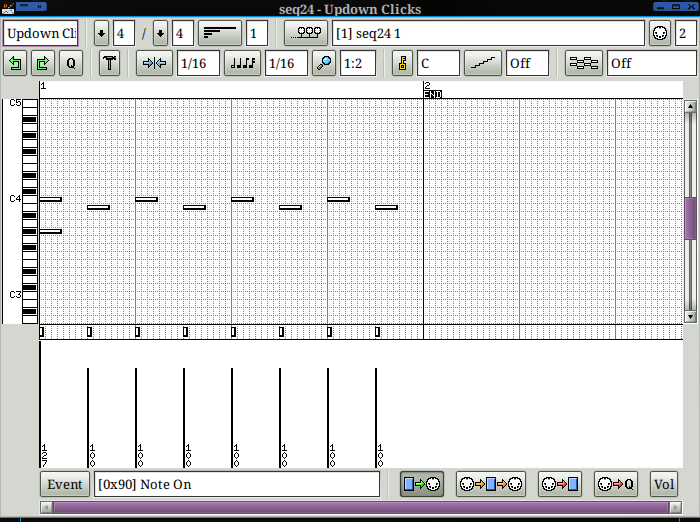
\includegraphics[scale=0.75]{pattern/pattern-edit-window.png}
   \caption{Pattern Edit Window}
   \label{fig:pattern_edit_window}
\end{figure}

   This dialog is quite complex.
   For exposition, we break it into a first panel, a second panel, a
   bottom panel, and a piano-roll/events section.

\subsection{Pattern Editor, First Panel}
\label{subsec:seq24_pattern_editor_first}

   TODO

\begin{figure}[H]
   \centering 
   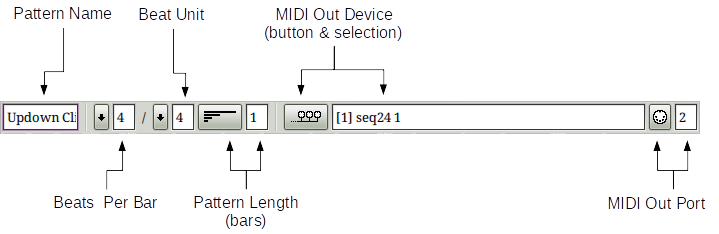
\includegraphics[scale=0.75]{pattern/pattern-edit-first-panel-items.png}
   \caption{Pattern Editor, First Panel Items}
   \label{fig:pattern_editor_first_panel_items}
\end{figure}

   TODO

\subsection{Pattern Editor, Second Panel}
\label{subsec:seq24_pattern_editor_second}

   TODO

\begin{figure}[H]
   \centering 
   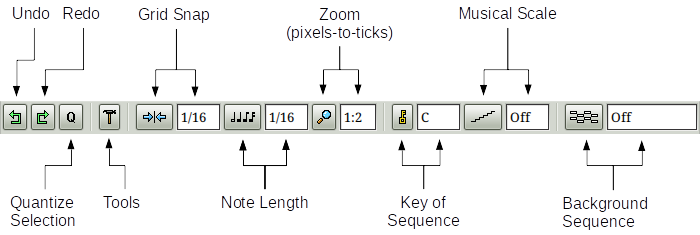
\includegraphics[scale=0.75]{pattern/pattern-edit-second-panel-items.png}
   \caption{Pattern Editor, Second Panel Items}
   \label{fig:pattern_editor_main_panel_items}
\end{figure}

   TODO

\subsection{Pattern Editor, Piano Roll}
\label{subsec:seq24_pattern_editor_piano_roll}

   TODO

\begin{figure}[H]
   \centering 
   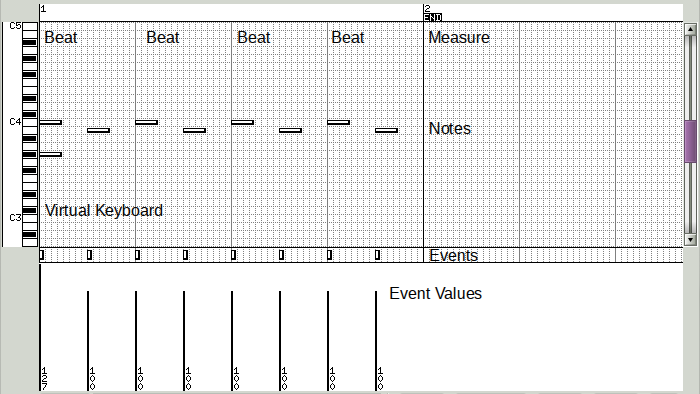
\includegraphics[scale=0.75]{pattern/pattern-edit-piano-roll-items.png}
   \caption{Pattern Editor, Piano Roll Items}
   \label{fig:pattern_editor_piano_roll_items}
\end{figure}

   TODO

\begin{figure}[H]
   \centering 
   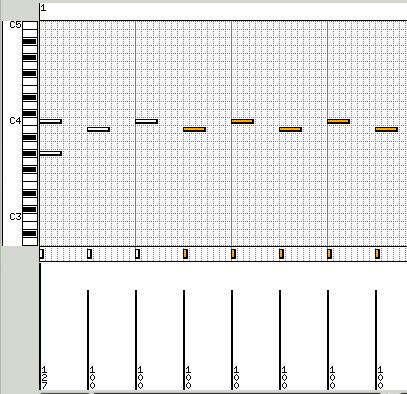
\includegraphics[scale=0.75]{pattern/pattern-edit-selected-events.png}
   \caption{Piano Roll, Selected Notes and Events}
   \label{fig:pattern_editor_selected_events}
\end{figure}

   TODO

\subsection{Pattern Editor, Bottom Panel}
\label{subsec:seq24_pattern_editor_bottom}

   TODO

\begin{figure}[H]
   \centering 
   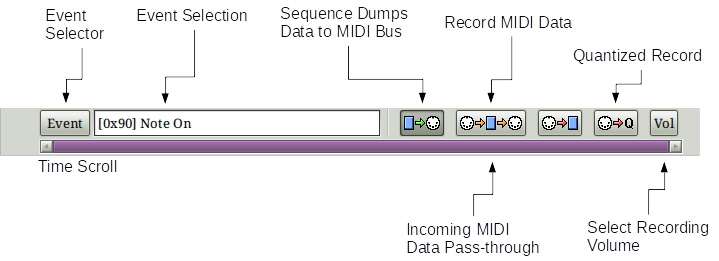
\includegraphics[scale=0.75]{pattern/pattern-edit-bottom-panel-items.png}
   \caption{Pattern Editor, Bottom Panel Items}
   \label{fig:pattern_editor_bottom_panel_items}
\end{figure}

   TODO


%-------------------------------------------------------------------------------
% vim: ts=3 sw=3 et ft=tex
%-------------------------------------------------------------------------------
